\documentclass[../main-notes.tex]{subfiles}

\begin{document}

\section{Parabola}

A parabola is the set of all points in the plane that are equidistant from a given line $L$, called directrix, and a given point $F$, called focus, which is not on le line $L$.
The distance between the directrix and the focus is $p=2a$, where $a$ is the distance from the vertex to the directrix or focus. (fig.\ref{fig-parabola})
\begin{marginfigure}
    \centering
    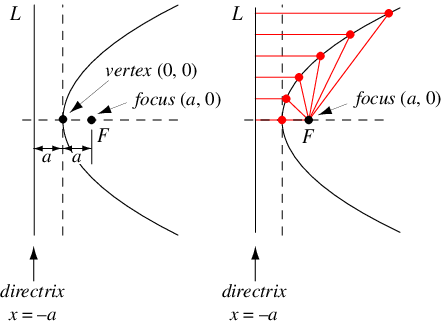
\includegraphics[width=\textwidth]{../Figures/parabola/ParabolaDirectrix_1001.png}
    \caption{The figure from the left are the gemetrical representation of the directrix, focus and vertex. On the right it is shown the distances from the focus to the parabola are equal from the point of the parabola to the directrix.}\label{fig-parabola}
\end{marginfigure}

\section{Derivation of the equation}

we are going to use the same tools from the last sessions.
Since the parabola is the set of all points in the plane that are equidistance from a given point and a given line, we use the distance function between two points and a distance between a point and a line.
The distance between the focus ($(0,a)$) and any other point in the plane is $d=\sqrt{(x-a)^2 + y^2}$.
Tacking into account the fig.\ref{fig-parabola}, the directrix is the vertical line $x=-a$, hence, the distance any point\footnote{In this distance we can ``ignore'' the $y$ component of the point, because we are only considereing perpendicular points from the directrix.} of the line to the vertex is $x+a$.

Now that we know the distances from any point of the plane to the focus and the distance from the directrix to the vertex, we can apply the equidistant restriction,
\begin{align*}
    \sqrt{(x-a)^2 + y^2} &= x+a.
\end{align*}
Now we are going to make some algebraic manipulations to get a more friendly expression,
\begin{align*}
    (x-a)^2 + y^2 &= \qty(x+a)^2 \\
    \cancelto{0}{x^2} -2ax +\cancelto{0}{a^2} + y^2 &= \cancelto{0}{x^2} +2ax +\cancelto{0}{a^2} \\
    y^2 &= 4ax. 
\end{align*}

\section{General equation}

As the other conic sections, we are going to consider the situation in which the vertex is not at the origin, as shown in figure\ref{fig-parabola}, instead is at an arbitrary point in the plane $(h,k)$.
Therefore\footnote{Please be \textbf{very} carefull with the parathensis, they are really important.},
\begin{gather*}
    \qty(y-k)^2 = 4a\qty(x-h).
\end{gather*}

\subsection{What if...}

Before moving on with the examples and exercises, it is important to consider the case in which the directrix is not a vertical line, but rather an horizontal one, and the focus is at $F=(0,a)$, not $F=(a,0)$.
Following the same procedure as before\footnote{
\begin{align*}
    \sqrt{x^2 + (y-a)^2} &= y+a \\
    x^2 + (y-a)^2 &= \qty(y+a)^2 \\
    x^2 + \cancelto{0}{y^2} -2ax +\cancelto{0}{a^2} &= \cancelto{0}{y^2} +2ay +\cancelto{0}{a^2} \\
    x^2 &= 4ay. 
\end{align*}
}
we get,
\begin{gather*}
    x^2 = 4ay.
\end{gather*}
Finally, to consider a vertex at any point in the plane,
\begin{gather*}
    \qty(x-h)^2 = 4a\qty(y-k).
\end{gather*}

\begin{note}{Expanded form}{~}
 \begin{align*}
    \qty(x-h)^2 &= 4a\qty(y-k) \\
    y^2 -2hx +h^2 &= 4ay-4ak \\
    \frac{1}{4a}\qty[4ay] &=\frac{1}{4a}\qty[-x^2 +2hx - h^2 -4ak] \\
    y &=-\frac{x^2}{4a} +\frac{hx}{2a} -\frac{h^2}{4a}  -k 
\end{align*}

In this case this function (a parabola with horizontal directrix) is bijective and has the following domain and range $x\in(-\infty,\infty)$ and $f(x,y)\in\qty(-\infty,\infty)$.
However, we need to be careful, because the parabola with a vertical directrix is not a bijective function, because for each value of $x$ it corresponds two values of $y$.
   
\end{note}

\subfile{exercise.tex}

\end{document}
